\problemname{Glyph Recognition}

You are an archaeologist working at an excavation site where your team
has found hundreds of clay tablets containing glyphs written in some
ancient language. Not much is known about the language yet, but you
know that there are only six different glyphs, each of them in the
shape of a regular polygon with one vertex pointing to the right (see
Figure~\ref{fig:alphabet} below). Only the boundary of each polygon is
carved out of the clay.

\begin{figure}[!h]
  \begin{subfigure}[t]{.23\textwidth}
    \centering
    \includegraphics[width=\textwidth]{alphabet.pdf}
    \caption{The six glyphs.}
    \label{fig:alphabet}
  \end{subfigure}%
  \begin{subfigure}[t]{.37\textwidth}
    \centering
    \includegraphics[width=.8\textwidth]{1-without.pdf}
    \caption{The first sample input.}
  \end{subfigure}%
  \begin{subfigure}[t]{.4\textwidth}
    \begin{minipage}{\textwidth}
      \vspace{-4.5cm}
      \includegraphics[width=.5\textwidth]{1-triangle.pdf}%
      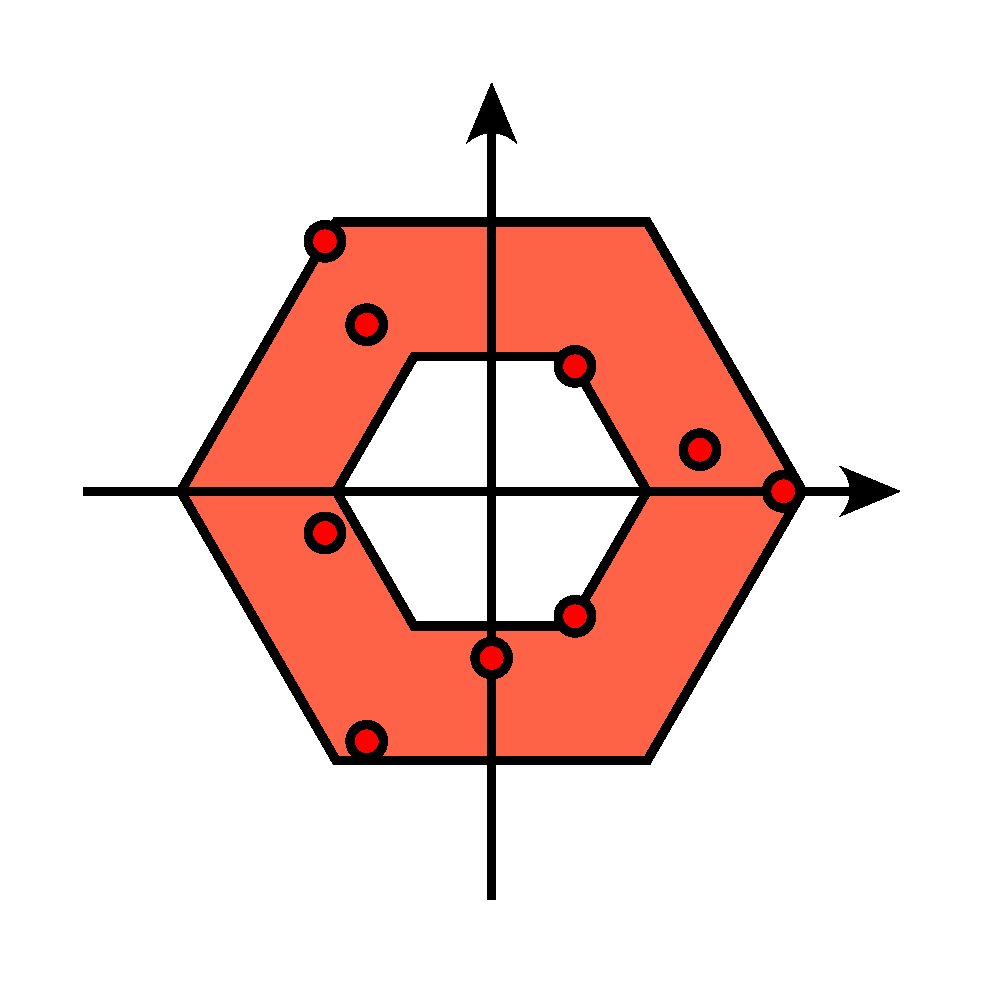
\includegraphics[width=.5\textwidth]{1-hexagon.pdf}
    \end{minipage}
    \centering
    \caption{Fitting triangles and hexagons to the first sample.
    The triangles' score is higher.}
    \label{fig:polyrec-sample}
  \end{subfigure}
  \caption{}
  \label{fig:polyrec}
\end{figure}

You want to start analysing the language right away, so you need to
get the text on the tablets into some machine readable format.
Ideally, you would like to use an OCR (optical character recognition)
tool for that, but you do not have one installed on your laptop and
there is no internet connection at the site.

Because of this you have devised your own scheme to digitise the
ancient writings: for every glyph on a tablet you first find a number
of sample points that are in the carved out region, i.e.~on the
boundary of the polygon. Based on those sample points you then
calculate a score for each of the six glyphs and mark the one with the
highest score as the recognised glyph.

%For a given number of corners $k$ ($3 \le k \le 8$), the score is
%computed as follows: two regular $k$-gons are fitted to the sample
%points, one from the inside and one from the outside. The two polygons
%are positioned such that they each have one vertex on the positive
%$x$-axis and all of their vertices have equal distance to the origin
%$(0,0)$ (see Figure~\ref{fig:polyrec-sample} above for an example).
%The score for that value of $k$ is then the ratio of the areas of the
%inner and outer polygons.

For a given number of corners $k$ ($3 \le k \le 8$), the score is
computed as follows. Two regular $k$-gons are fitted to the sample
points, one from the inside and one from the outside, such that the
following hold:

\begin{itemize}
  \item Each polygon is centered at the origin, i.e.~all vertices have
  equal distance to $(0,0)$.
  \item Each polygon has a vertex on the positive $x$-axis.
  \item The inner polygon is the largest such polygon containing none
  of the sample points.
  \item The outer polygon is the smallest such polygon containing all
  of the sample points.
\end{itemize}

An example can be seen in Figure~\ref{fig:polyrec-sample}.
The score for this value of $k$ is $\frac{A_\text{inner}}{A_\text{outer}}$,
where $A_\text{inner}$ and $A_\text{outer}$ are the areas of the inner and
outer polygon, respectively.

Given a set of sample points, find the glyph with the highest score.

\section*{Input}

The input consists of:
\begin{itemize}
	\item One line with one integer $n$ ($1 \le n \le 1\,000$), the
    number of sample points.
  \item $n$ lines, each with two integers $x,y$ ($-10^6 \le x,y
    \le 10^6$), specifying a point at coordinates $(x,y)$.
\end{itemize}
No sample point is at the origin and all points are distinct.

\section*{Output}

Output the optimal number of corners $k$ ($3 \le k \le 8$), followed
by the score obtained for that value of $k$. Your answer will be
accepted if the absolute error does not exceed $10^{-6}$. If several
values of $k$ result in a score that is within $10^{-6}$ of the
optimal score, any one of them will be accepted.
